% Compile with pdfLaTeX twice, latexmk -pdf, or Tectonic.
% Keep the figures/ folder beside this file. No BibTeX or shell escape needed.
\documentclass[11pt,a4paper]{article}
\usepackage[T1]{fontenc}
\usepackage{lmodern}
\usepackage[margin=23mm,headheight=15pt]{geometry}
\usepackage{amsmath,amssymb,mathtools,bm}
\usepackage{microtype}
\usepackage{xcolor,graphicx}
\usepackage{booktabs,tabularx,array}
\usepackage{enumitem}
\usepackage{float}
\usepackage{placeins}
\usepackage{tikz}
\usetikzlibrary{arrows.meta,positioning}
\usepackage{fancyhdr}
\usepackage{hyperref}
\usepackage{bookmark}
\definecolor{ink}{HTML}{17354C}
\definecolor{teal}{HTML}{087E8B}
\definecolor{rust}{HTML}{A84429}
\hypersetup{colorlinks=true,linkcolor=ink,citecolor=teal,urlcolor=teal,
 pdftitle={From Maxwell's Equations to Lithographic Imaging}}
\graphicspath{{figures/}}
\pagestyle{fancy}
\fancyhf{}
\fancyfoot[C]{\thepage}
\renewcommand{\headrulewidth}{0.3pt}
\setlength{\parindent}{0pt}
\setlength{\parskip}{5pt plus 1pt}
\setlength{\emergencystretch}{2em}
\renewcommand{\topfraction}{.9}
\renewcommand{\textfraction}{.08}
\renewcommand{\floatpagefraction}{.75}
\setlist{itemsep=2pt,topsep=4pt}
\allowdisplaybreaks[2]
\numberwithin{equation}{section}
\newcommand{\dd}{\mathrm{d}}
\newcommand{\ii}{\mathrm{i}}
\newcommand{\ee}{\mathrm{e}}
\newcommand{\vct}[1]{\bm{#1}}
\newcommand{\avg}[1]{\left\langle #1\right\rangle}
\newcommand{\FT}{\mathcal F}
\newcommand{\NA}{\mathrm{NA}}
\newcommand{\Real}{\operatorname{Re}}
\newcommand{\nm}{\,\mathrm{nm}}
\newcommand{\um}{\,\mu\mathrm m}
\newcommand{\design}[1]{\par\smallskip{\color{teal}\textbf{Design connection.}} #1\par\smallskip}
\newcommand{\keep}[1]{\par\smallskip{\color{rust}\textbf{Keep distinct.}} #1\par\smallskip}
\newcolumntype{Y}{>{\raggedright\arraybackslash}X}

\begin{document}
{\LARGE\color{ink}\bfseries From Maxwell's Equations to Lithographic Imaging\par}

\vspace{5mm}

\textbf{Conventions Through The Document.} Time dependence is $\ee^{-\ii\omega t}$, $\lambda_0$
is the vacuum wavelength, and $\lambda_m=\lambda_0/n$ is the wavelength
in a lossless medium. Transverse coordinates are $\vct x=(x,y)$;
$\vct f=(f_x,f_y)$ is spatial frequency in \emph{cycles per unit length}.
Except where a refractive index is explicitly retained, the diffraction
and imaging calculations below use vacuum or air, with
$n=1$, $\lambda=\lambda_0$, and $k=2\pi/\lambda$.

\section{From Maxwell's equations to the intensity we measure}
\subsection{The wave equation and the meaning of a complex field}
In a linear, isotropic medium, $\vct D=\epsilon\vct E$ and
$\vct B=\mu\vct H$. Maxwell's equations for the \emph{real} fields are
\begin{align}
\nabla\cdot(\epsilon\vct E)&=\rho_{\rm free},&
\nabla\cdot(\mu\vct H)&=0,\notag\\
\nabla\times\vct E&=-\mu\partial_t\vct H,&
\nabla\times\vct H&=\vct J_{\rm free}+\epsilon\partial_t\vct E.
\end{align}
The physical source involves charges and currents. In a homogeneous,
source-free propagation region, set $\rho_{\rm free}=0$,
$\vct J_{\rm free}=0$, and take $\epsilon,\mu$ constant. Taking a curl,
\begin{align}
\nabla\times(\nabla\times\vct E)
&=-\mu\partial_t(\nabla\times\vct H)
=-\mu\epsilon\partial_t^2\vct E,\notag\\
\nabla(\nabla\cdot\vct E)-\nabla^2\vct E
&=-\mu\epsilon\partial_t^2\vct E
\quad\Longrightarrow\quad
\boxed{\nabla^2\vct E-\mu\epsilon\partial_t^2\vct E=0.}
\end{align}
For one optical frequency, introduce a spatial phasor
$\widetilde{\vct E}$:
\begin{equation}
\vct E(\vct r,t)=\Real\{\widetilde{\vct E}(\vct r)\ee^{-\ii\omega t}\},
\qquad
\boxed{(\nabla^2+k_m^2)\widetilde{\vct E}=0,\quad
k_m=\omega\sqrt{\mu\epsilon}=\frac{2\pi n}{\lambda_0}.}
\label{eq:helmholtz}
\end{equation}
The second time derivative supplies $-\omega^2$. Equation
\eqref{eq:helmholtz} is the vector Helmholtz equation. Its components
satisfy scalar Helmholtz equations in this homogeneous region, but also
obey the Maxwell constraint $\nabla\cdot\widetilde{\vct E}=0$.
For a common, approximately fixed polarization we use one scalar phasor
$\mathcal E$ through $\widetilde{\vct E}=\widehat{\vct e}\,\mathcal E$.
This scalar imaging approximation needs revision when polarization and
longitudinal-field effects matter.

\subsection{Why is it that \texorpdfstring{$I\propto|\mathcal E|^2$}{intensity proportional to field squared}}
Intensity is averaged energy flux, so begin with
$\vct S=\vct E\times\vct H$. For a travelling plane wave in a lossless
medium, Faraday's law relates its phasors:
\begin{equation}
\vct k\times\widetilde{\vct E}=\omega\mu\widetilde{\vct H},
\qquad
\widetilde{\vct H}=\frac{1}{\eta}\widehat{\vct s}\times\widetilde{\vct E},
\qquad \eta=\sqrt{\mu/\epsilon}.
\end{equation}
Here $\widehat{\vct s}$ is the propagation direction and
$\widehat{\vct s}\cdot\widetilde{\vct E}=0$. For linear polarization,
$\mathcal E=A\ee^{\ii\phi}$ gives the particularly transparent check
\begin{equation}
E=A\cos(\phi-\omega t),\qquad
S_{\parallel}=\frac{A^2}{\eta}\cos^2(\phi-\omega t),\qquad
\boxed{I=\avg{S_{\parallel}}_{\rm optical}
=\frac{A^2}{2\eta}=\frac{|\mathcal E|^2}{2\eta}.}
\label{eq:intensity}
\end{equation}
Thus the factor $1/2$ comes from the optical-cycle average, and $1/\eta$
from the magnetic-to-electric-field relation. Equivalently, using
$E=(\mathcal E\ee^{-\ii\omega t}+\mathcal E^*\ee^{\ii\omega t})/2$,
\[
\avg{E^2}_{\rm optical}
=\frac14\avg{\mathcal E^2\ee^{-2\ii\omega t}
+2|\mathcal E|^2+(\mathcal E^*)^2\ee^{2\ii\omega t}}
=\frac12|\mathcal E|^2.
\]
These are \emph{peak} phasor amplitudes; an RMS amplitude already includes
the factor $1/\sqrt2$. In a nonmagnetic dielectric,
$1/\eta=n\epsilon_0c$, so $I=n\epsilon_0c|\mathcal E|^2/2$.
The general monochromatic flux formula is
$\avg{\vct S}_{\rm optical}=\tfrac12\Real
(\widetilde{\vct E}\times\widetilde{\vct H}^{\,*})$.
It remains the appropriate starting point for vector, absorbing, or
standing-wave fields where the simple travelling-wave reduction is inadequate.

\subsection{Exactly how \texorpdfstring{$E$ and $U$}{E and U} are linked}
We use an intensity-normalized scalar amplitude throughout the rest of
these notes:
\begin{equation}
\boxed{U=\frac{\mathcal E}{\sqrt{2\eta}},\qquad
E(\vct r,t)=\Real\{\sqrt{2\eta}\,U(\vct r)\ee^{-\ii\omega t}\},
\qquad I=|U|^2.}
\label{eq:normalization}
\end{equation}
Here $E$ is the real field component along the chosen linear polarization.
$\mathcal E$ is measured in $\mathrm{V/m}$; $U$ is measured in
$\sqrt{\mathrm W}/\mathrm m$. Multiplying by a constant does not change
the homogeneous Helmholtz equation, so $U$ satisfies it too.
An alternative convention calls the unscaled phasor itself $U$, in which
case $I=|U|^2/(2\eta)$. The convention must be stated once and kept consistent.

For a fluctuating narrowband source, write a slowly varying amplitude
$U(\vct r,\tau)$ and then measure
$I=\avg{|U|^2}_{\rm exposure}$. Optical-cycle averaging and averaging
relative-phase fluctuations are separate steps; the latter determines
coherence. A source can therefore be described downstream by its field
or its field correlations on a chosen plane, without solving its
microscopic emission process each time. See Born--Wolf and
Saleh--Teich for the electromagnetic and scalar-wave foundations
\cite{bw,st}.

\subsection{Helmholtz equation}
\label{sec:helmholtz-derivation}
We can now make the transition from the real electric field to the
spatial equation for $U$ explicit. Retain a homogeneous, source-free,
linear, isotropic, lossless medium, with constant $\epsilon$ and $\mu$.
The wave equation applies to each Cartesian electric-field component;
representing the whole field by one scalar additionally uses the
polarization approximation described above.

\textbf{1. Start from the time-dependent Maxwell equation.}
Taking the curl of Faraday's law and using the source-free Ampere law
gives $\nabla\times(\nabla\times\vct E)
=-\mu\epsilon\partial_t^2\vct E$. Since constant $\epsilon$ and
$\nabla\cdot(\epsilon\vct E)=0$ imply $\nabla\cdot\vct E=0$, the
curl--curl identity gives, for a real component $E$,
\begin{equation}
\boxed{\nabla^2E-\frac{1}{v^2}\frac{\partial^2E}{\partial t^2}=0,}
\qquad v=\frac{1}{\sqrt{\mu\epsilon}}=\frac{c}{n}.
\label{eq:real-scalar-wave}
\end{equation}

\textbf{2. Separate the single-frequency time dependence.}
For a monochromatic field, define the complex representation
\begin{equation}
E_{\rm c}(\vct r,t)=\mathcal E(\vct r)\ee^{-\ii\omega t}
=\sqrt{2\eta}\,U(\vct r)\ee^{-\ii\omega t},
\qquad E=\Real E_{\rm c}.
\label{eq:helmholtz-ansatz}
\end{equation}
The subscript $\rm c$ marks the complex representation. The phasor $U(\vct r)$
has no time dependence for this one frequency, but its amplitude and
phase may both vary with position.

\textbf{3. Evaluate the derivatives separately.}
Because $\eta$ is spatially constant in this medium,
\begin{align}
\nabla^2E_{\rm c}
&=\sqrt{2\eta}\,\ee^{-\ii\omega t}\nabla^2U,\notag\\
\frac{\partial^2 E_{\rm c}}{\partial t^2}
&=\sqrt{2\eta}\,U(-\ii\omega)^2\ee^{-\ii\omega t}
=-\omega^2\sqrt{2\eta}\,U\ee^{-\ii\omega t}.
\label{eq:helmholtz-derivatives}
\end{align}
The Laplacian differentiates the spatial phasor; the time derivatives
act only on the exponential term.

\textbf{4. Substitute and cancel the common factor.}
Insert Eq.~\eqref{eq:helmholtz-derivatives} into
Eq.~\eqref{eq:real-scalar-wave}, using its complex representation:
\[
0=\sqrt{2\eta}\,\ee^{-\ii\omega t}
\left[\nabla^2U+\frac{\omega^2}{v^2}U\right].
\]
The prefactor is nonzero, so the bracket must vanish. Define the
wave number in the medium by
\begin{equation}
k_m=\frac{\omega}{v}=\frac{n\omega}{c}
=nk_0=\frac{2\pi}{\lambda_m},\qquad
k_0=\frac{\omega}{c}=\frac{2\pi}{\lambda_0}.
\end{equation}
We obtain the scalar Helmholtz equation,
\begin{equation}
\boxed{\nabla^2U+k_m^2U=0,\qquad\text{or}\qquad
\nabla^2U+n^2k_0^2U=0.}
\label{eq:scalar-helmholtz}
\end{equation}
For example, in Cartesian coordinates this means
$\partial_x^2U+\partial_y^2U+\partial_z^2U+k_m^2U=0$.
The unscaled phasor $\mathcal E=\sqrt{2\eta}\,U$ obeys the same
equation because the normalization is constant.

\textbf{5. Check the result with a plane wave.}
Let $U=U_0\ee^{\ii(k_xx+k_yy+k_zz)}$. Each second spatial derivative
supplies a minus sign, giving
\begin{equation}
\nabla^2U=-(k_x^2+k_y^2+k_z^2)U
\quad\Longrightarrow\quad
k_x^2+k_y^2+k_z^2=k_m^2.
\label{eq:helmholtz-plane-wave-check}
\end{equation}
For a propagating plane wave with a real wavevector,
$|\vct k|=k_m=2\pi/\lambda_m$, as expected. 

% Solving this relation for
% $k_z$ will give the angular-spectrum propagation rule below.

% Helmholtz describes the spatial amplitude and phase at one fixed optical
% frequency; the real field still oscillates through the carrier in
% Eq.~\eqref{eq:helmholtz-ansatz}. No paraxial or small-angle approximation
% was used in the passage from the wave equation to Helmholtz. Those
% approximations enter later when simplifying propagation. For a
% superposition of frequencies, apply the equation to each frequency
% component; interfaces and spatially varying materials require the
% appropriate Maxwell equations and boundary conditions.

\section{After the source: pupils, spatial frequencies, and propagation}
\subsection{What each part of the optical system does}
\begin{center}
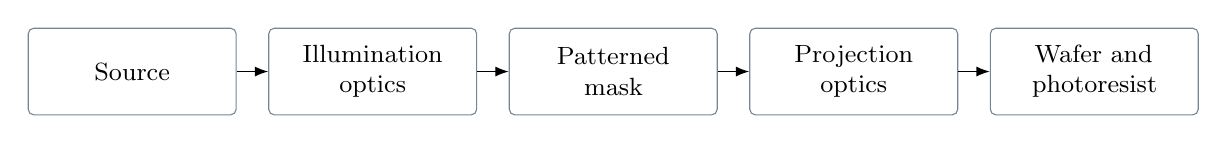
\begin{tikzpicture}[>=Latex, node distance=4mm,
 box/.style={draw=ink!60,rounded corners=2pt,align=center,
 font=\small,minimum height=11mm,text width=25mm,inner sep=2pt}]
\node[box] (s) {Source};
\node[box,right=of s] (i) {Illumination\\optics};
\node[box,right=of i] (m) {Patterned\\mask};
\node[box,right=of m] (p) {Projection\\optics};
\node[box,right=of p] (w) {Wafer and\\photoresist};
\draw[->] (s)--(i);\draw[->] (i)--(m);\draw[->] (m)--(p);\draw[->] (p)--(w);
\end{tikzpicture}
\end{center}
The aperture stop limits the accepted ray cone. Its images through the
preceding and following optics are the \emph{entrance} and \emph{exit}
pupils.
For an image-side cone of half-angle $\alpha_{\max}$,
\begin{equation}
\NA=n\sin\alpha_{\max},\qquad
f_c=\frac{\NA}{\lambda_0}.
\label{eq:cutoff}
\end{equation}
NA is dimensionless; $f_c$ is a field spatial-frequency cutoff.
The illumination optics determine which directions reach the mask.
The projection pupil determines which outgoing components the projector
admits. A source distribution and a projection pupil are different objects.

For a thin scalar mask with complex amplitude transmission or reflection
$t(\vct x)$, the field just after the mask is
\begin{equation}
U_o(\vct x)=t(\vct x)U_{\rm inc}(\vct x).
\label{eq:mask}
\end{equation}
Later, the imaging optics apply their own amplitude and phase response.
Mask reflectance belongs in $t$; projection-mirror losses belong in the
system response. They do not count the same reflection twice.
Setting $U_{\rm inc}=1$ assumes a spatially constant coherent field and
chooses its amplitude as the unit. \emph{Normalization, uniformity, and
coherence are independent concepts.}

\subsection{The pupils are the apparent stop}
\label{sec:two-lens-pupils}
Imagine looking into the two-lens system in
Fig.~\ref{fig:two-lens-pupils} from each end.
From the \textbf{left}, lens $L_1$ makes the stop appear larger and at a
different position: this apparent opening is the \textbf{entrance pupil
(EP)}. From the \textbf{right}, lens $L_2$ gives another apparent size
and position: the \textbf{exit pupil (XP)}. Both are images of the same
physical stop \cite{bw,st}.

\begin{figure}[H]
\centering
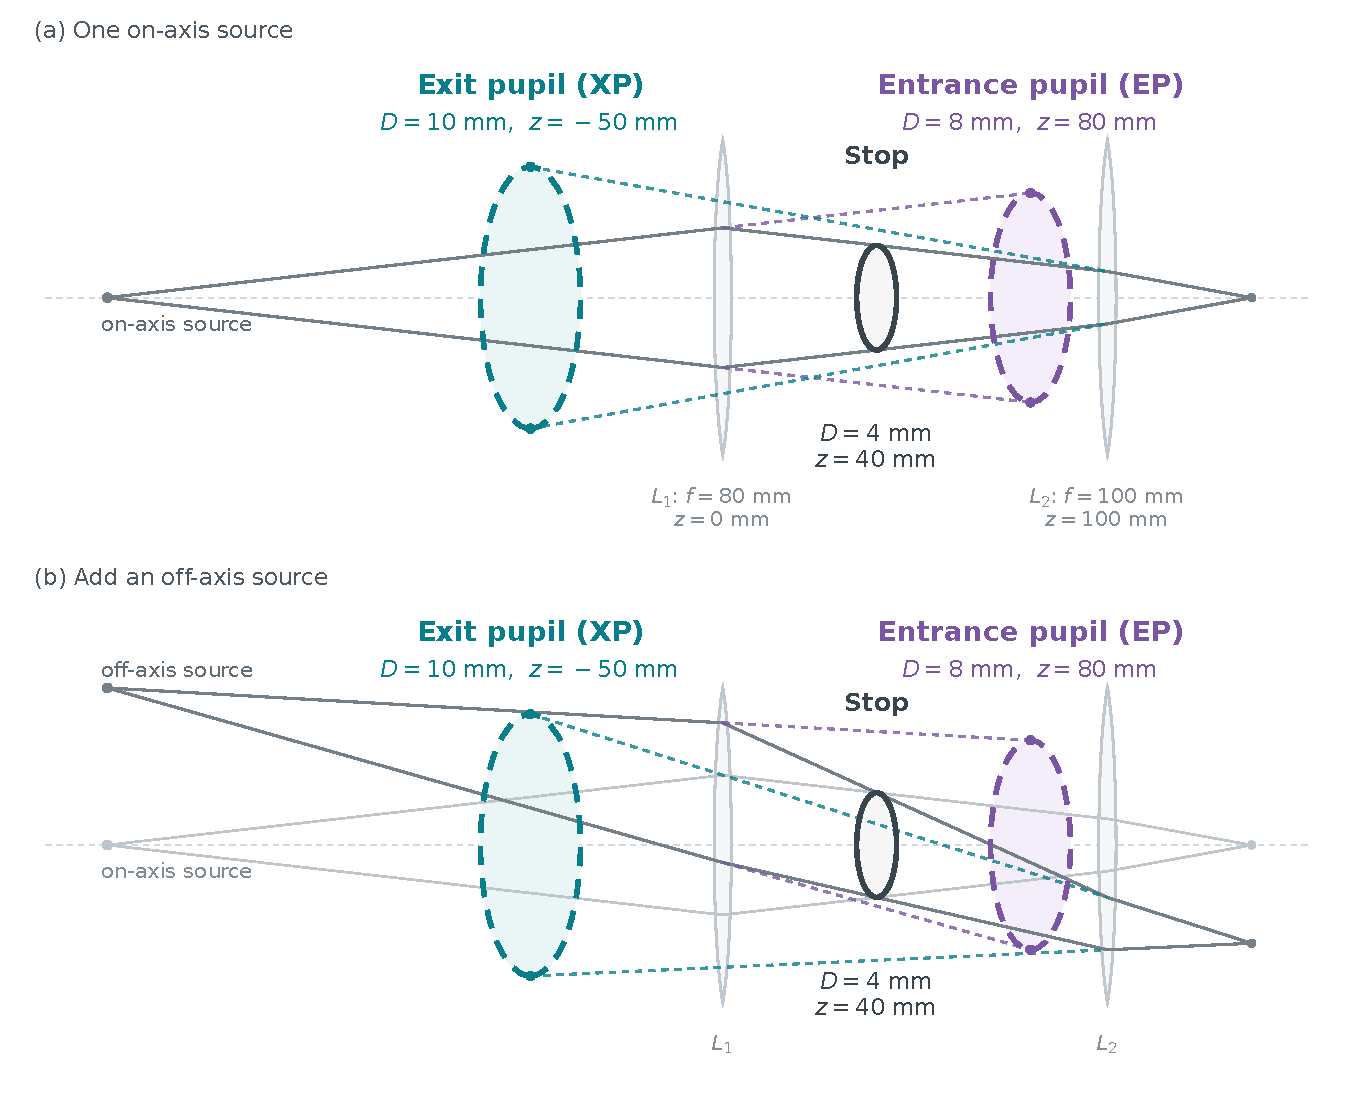
\includegraphics[width=\textwidth]{two_lens_pupils.pdf}
\caption{Pupil position and diameter $D$ for (a) one on-axis source and
(b) an added off-axis source. Thin solid rays pass through the stop.
Purple dashed extensions of the incoming rays meet the EP edges;
teal dashed extensions of the outgoing rays meet the XP edges.
The coloured openings are virtual images of the physical stop.
Both sources share the same pupils. Diameters share one vertical
scale; axial distances use a different scale.}
\label{fig:two-lens-pupils}
\end{figure}

The names \emph{entrance} and \emph{exit} refer to the viewing side. 

The entrance pupil describes the opening seen from the mask.
The exit pupil's diameter and distance from the wafer determine the
image-side cone angle, and hence the Numerical Aperture and cutoff spatial frequency.

\subsection{A spatial frequency is variation across a fixed plane}
Use the transverse Fourier pair
\begin{equation}
\widetilde U(\vct f,z)=\int U(\vct x,z)\ee^{-\ii2\pi\vct f\cdot\vct x}\dd^2x,
\qquad
U(\vct x,z)=\int\widetilde U(\vct f,z)\ee^{\ii2\pi\vct f\cdot\vct x}\dd^2f.
\label{eq:fourier}
\end{equation}
For a plane wave tilted towards $x$ by $\theta$ in a lossless medium,
\[
U(x,z)=U_0\exp\!\left[\ii\frac{2\pi n}{\lambda_0}
(x\sin\theta+z\cos\theta)\right]
\quad\Longrightarrow\quad f_x=\frac{n\sin\theta}{\lambda_0}.
\]
Larger tilt means faster phase variation across the \emph{fixed}
$z=\text{constant}$ plane. %That plane generally cuts across several wavefronts; a wavefront itself has constant phase. 
% The components of
% $\vct k$ describe direction, while the components of $\vct E$ describe
% polarization. The scalar $U$ is not a vector with ``propagation, $x$, and
% $y$'' components.

A fine mask pattern has large spatial frequencies in their transmittance/reflectance. Under normal,
uniform illumination these also appear in $U_o$. Oblique illumination
$\ee^{\ii2\pi\vct s\cdot\vct x}$ shifts the field spectrum to
$\widetilde t(\vct f-\vct s)$. The intensity $|U|^2$ has its own
frequencies, which are differences between field frequencies.

\subsection{Exact propagation and evanescent components}
Fourier-transform the transverse derivatives in Helmholtz equation:
\begin{equation}
\partial_z^2\widetilde U+
\left[k_m^2-(2\pi)^2|\vct f|^2\right]\widetilde U=0.
\end{equation}
For outgoing propagation into $z>0$, choose the forward or decaying branch:
\begin{align}
\widetilde U(\vct f,z)&=H_z(\vct f)\widetilde U(\vct f,0),\notag\\
H_z(\vct f)&=\ee^{\ii k_z z},\qquad
k_z=\sqrt{k_m^2-(2\pi)^2|\vct f|^2},\quad
\Real k_z\geq0,\quad\operatorname{Im}k_z\geq0.
\label{eq:angular}
\end{align}
Substituting $k_m=2\pi n/\lambda_0$ gives the \textbf{exact propagation
transfer function} explicitly:
\begin{equation}
\boxed{H_z(f_x,f_y)=\exp\!\left[
\ii 2\pi z\sqrt{\left(\frac{n}{\lambda_0}\right)^2-f_x^2-f_y^2}
\right].}
\label{eq:exact-propagator}
\end{equation}
In vacuum, $n=1$, $\lambda=\lambda_0$, and $k=2\pi/\lambda$, so this is
\[
H_z(\vct f)=\exp\!\left[\ii kz\sqrt{1-\lambda^2|\vct f|^2}\right].
\]
The full square root is retained. Multiplying the input spectrum by
$H_z$ and taking the inverse transverse Fourier transform gives
\begin{equation}
U(\vct x,z)=\FT^{-1}\!\left[
H_z(\vct f)\widetilde U(\vct f,0)\right](\vct x).
\label{eq:exact-field-propagation}
\end{equation}
For $|\vct f|<n/\lambda_0$, $k_z$ is real: the component propagates,
and $H_z$ changes its phase. For $|\vct f|>n/\lambda_0$,
\begin{equation}
k_z=\ii\kappa,\qquad
\kappa=2\pi\sqrt{|\vct f|^2-(n/\lambda_0)^2},\qquad
H_z=\ee^{-\kappa z}.
\end{equation}
This is an evanescent component, with amplitude decay length $1/\kappa$.
It still satisfies $\vct k\cdot\vct k=k_m^2$; the wavevector is complex,
so the real-vector bound $|\vct k_\perp|\leq k_m$ no longer applies.
The equality $|\vct f|=n/\lambda_0$ is the grazing boundary, $k_z=0$.

\begin{center}
\small
\begin{tabularx}{\textwidth}{@{}lY@{}}
\toprule Transverse frequency & Meaning for a clear circular pupil\\\midrule
$|\vct f|\leq f_c$ & Within the pupil's angular acceptance.\\
$f_c<|\vct f|<n/\lambda_0$ & Propagating, but rejected by this pupil.\\
$|\vct f|>n/\lambda_0$ & Evanescent in this medium.\\\bottomrule
\end{tabularx}
\end{center}
% Since $f_c=n\sin\alpha_{\max}/\lambda_0\leq n/\lambda_0$, an immersion
% NA above one does not imply collecting evanescent components in the
% immersion medium. Its propagation limit rises too.
A sharp edge requires a wide range of field frequencies: some propagate
and are rejected by the pupil, while sufficiently high ones are confined
near the edge. Both mechanisms limit transferred detail, for different reasons.

\subsection{Fresnel propagation is an approximation to this result}
In vacuum, expand the square root for $\lambda|\vct f|\ll1$:
\begin{align}
k_z&=k\sqrt{1-\lambda^2|\vct f|^2}
\simeq k-\pi\lambda|\vct f|^2,\notag\\
H_z(\vct f)&\simeq\ee^{\ii kz}\ee^{-\ii\pi\lambda z|\vct f|^2}.
\label{eq:fresnel-transfer}
\end{align}
Inverse transformation gives the convolution with a quadratic-phase kernel:
\begin{equation}
\boxed{U(\vct x,z)=\frac{\ee^{\ii kz}}{\ii\lambda z}
\int U(\vct x',0)
\exp\!\left[\frac{\ii\pi|\vct x-\vct x'|^2}{\lambda z}\right]\dd^2x'.}
\label{eq:fresnel}
\end{equation}
% For completeness, each one-dimensional inverse transform uses the Fresnel
% Gaussian integral
% \[
% \int_{-\infty}^{\infty}\ee^{-\ii\pi a f^2+\ii2\pi b f}\dd f
% =\frac{\ee^{-\ii\pi/4}}{\sqrt a}\ee^{\ii\pi b^2/a},\qquad a>0.
% \]
% The two transverse dimensions supply $\ee^{-\ii\pi/2}/(\lambda z)
% =1/(\ii\lambda z)$. Equivalently, expand a propagation distance as
% $R\simeq z+|\vct x-\vct x'|^2/(2z)$ and approximate $1/R$ by $1/z$.
% The omitted angular-spectrum phase is approximately
% \begin{equation}
% |\Delta\phi|\simeq\frac{\pi z\lambda^3}{4}|\vct f|^4.
% \label{eq:fresnel-error}
% \end{equation}
% Small angle alone is not a numerical error bound: this accumulated phase
% must also be small enough for the intended calculation.
% Unlike Eq.~\eqref{eq:exact-propagator}, the Fresnel transfer has unit modulus for
% every frequency and cannot describe evanescent decay.

The plane called $z=0$ is whichever input plane has a known field. 
Free propagation applies between optical elements.
Reflection, refraction, masks, and coatings require their own boundary
conditions or transfer factors. In a folded mirror train, a local axis
may be chosen for each propagation segment.

% If the input has characteristic radius $a$, the further far-field
% condition $a^2/(\lambda z)\ll1$ allows us to drop its quadratic phase:
% \[
% U(\vct x,z)\simeq\frac{\ee^{\ii kz}}{\ii\lambda z}
% \ee^{\ii\pi|\vct x|^2/(\lambda z)}
% \widetilde U\!\left(\frac{\vct x}{\lambda z},0\right).
% \]
% This is Fraunhofer diffraction. Focusing optics can instead cancel the
% quadratic phase, producing a Fourier-related plane at a finite distance.

The scalar angular spectrum is exact for its homogeneous,
source-free model, not for a complete scanner. Fresnel propagation is
useful for suitable paraxial segments; \emph{high-angle fields and the material
interfaces of an EUV mask can require vector Maxwell calculations}.

\section{How focusing and aberrations enter the point-spread function}
\subsection{The three phase terms that cancel at focus}
Consider a thin lens in air with focal length $F$, object distance $s_o$,
image distance $s_i$, and pupil coordinate $\vct\xi$.
For an on-axis object and on-axis observation point, the pupil-dependent
phases are
\begin{equation}
\underbrace{\frac{k|\vct\xi|^2}{2s_o}}_{\text{object to lens}}
\;\underbrace{-\frac{k|\vct\xi|^2}{2F}}_{\text{lens}}
\;\underbrace{+\frac{k|\vct\xi|^2}{2s_i}}_{\text{lens to image}}
=\frac{k|\vct\xi|^2}{2}
\left(\frac1{s_o}+\frac1{s_i}-\frac1F\right).
\label{eq:three-phases}
\end{equation}
% The propagation terms follow from
% $\sqrt{s^2+|\vct\xi|^2}\simeq s+|\vct\xi|^2/(2s)$.
% The lens's thickness profile supplies the opposing phase, relative to
% its centre. 
When $1/s_o+1/s_i=1/F$, the path-dependent phase vanishes:
contributions from all pupil positions arrive in phase at the image point.
% Immediately after the lens, the remaining phase is
% $-k|\vct\xi|^2/(2s_i)$, the phase of a converging wave.

\subsection{Point Spread Function and Optical Transfer Function }
Let $B(\vct\xi)$ contain the aperture, amplitude weighting, and residual
phase error, while the ideal lens phase has already been written explicitly.
For an object point at $\vct x_o$ and an image-plane coordinate $\vct x$,
the Fresnel calculation is
\begin{equation}
U_i(\vct x;\vct x_o)\propto
\int B(\vct\xi)\exp\!\left\{\frac{\ii k}{2}
\left[\frac{|\vct\xi-\vct x_o|^2}{s_o}
-\frac{|\vct\xi|^2}{F}
+\frac{|\vct x-\vct\xi|^2}{s_i}\right]\right\}\dd^2\xi.
\label{eq:point-integral}
\end{equation}
Expand the squares. At the imaging condition, the $|\vct\xi|^2$ term
cancels, leaving a pupil-independent phase
$\Phi_0=k(|\vct x_o|^2/s_o+|\vct x|^2/s_i)/2$ and
\begin{equation}
U_i\propto\ee^{\ii\Phi_0}
\int B(\vct\xi)
\ee^{-\ii2\pi\vct\xi\cdot(\vct x-M\vct x_o)/(\lambda s_i)}\dd^2\xi,
\qquad M=-\frac{s_i}{s_o}.
\end{equation}
Use reference-sphere field envelopes to remove these known ideal
quadratic phases, and absorb constant gains and the coordinate Jacobian
in the field convention. With the pupil-axis convention
$\vct f=-\vct\xi/(\lambda s_i)$, the result is
\begin{equation}
\boxed{h(\vct x)=\int P(\vct f)\ee^{\ii2\pi\vct f\cdot\vct x}\dd^2f
=\FT^{-1}[P](\vct x),\qquad
h_j(\vct x)=h(\vct x-M\vct x_{o,j}).}
\label{eq:psf}
\end{equation}
$h$ is the \emph{amplitude} point-spread function (PSF): the image field
from a unit point object. Its argument is a transverse image-plane
displacement, not a propagation distance. The pupil integration variable
$\vct f$ has inverse-length units; the condition is $|\vct f|\leq f_c$,
not $|\vct x|\leq f_c$.

For a circular pupil of physical radius $a$, the paraxial mapping gives
$f_c\simeq a/(\lambda s_i)=\NA/\lambda$. In the usual scalar pupil model,
\begin{equation}
\boxed{P(\vct f)=A(\vct f)\,
\mathbf1_{|\vct f|\leq f_c}\,
\exp\!\left[\frac{\ii2\pi}{\lambda}
W\!\left(\frac{\vct f}{f_c}\right)\right].}
\label{eq:pupil}
\end{equation}
$A\geq0$ describes amplitude attenuation or apodization; $W$ is
phase-equivalent optical path error relative to ideal imaging, including
any residual coating phase assigned to the projector.
The disk describes the support only: an aberrated $P$ is a \emph{complex
function on that disk}. Other pupil shapes give other supports.

% \keep{For an ideal clear system, $P=1$ inside the disk means zero
% \emph{residual} phase error. The lens or mirrors and their focusing action
% are already included in Eq.~\eqref{eq:psf}. A bare hole followed by
% arbitrary free propagation is a different optical system.}

Within a region where the system is approximately shift invariant,
superposition gives, in image-equivalent object coordinates,
\begin{equation}
\boxed{U_i=h*U_o=\FT^{-1}[P\widetilde U_o],\qquad
I_{\rm coh}=|U_i|^2.}
\label{eq:coherent}
\end{equation}
If $U_{\rm inc}=1$, then $U_o=t$ and $\widetilde U_o=\widetilde t$.
$\widetilde t$ describes which field components the mask supplies;
$P$ describes how the projector changes them. For physical mask
coordinates, first apply the magnification and orientation mapping.
In a 4:1 reduction, $|M|=1/4$; an image frequency is four times the
corresponding physical mask frequency.

\subsection{The Airy pattern and what an aberration changes}
For a clear, uniformly weighted circular pupil, $P=1$ within $f_c$.
Writing $r=|\vct x|$ and using polar pupil coordinates,
\begin{align}
h(r)&=\int_0^{f_c} f\,\dd f\int_0^{2\pi}
\ee^{\ii2\pi fr\cos\theta}\dd\theta
=2\pi\int_0^{f_c}fJ_0(2\pi fr)\dd f\notag\\
&=\frac{f_cJ_1(2\pi f_cr)}{r},\qquad h(0)=\pi f_c^2.
\end{align}
The angular integral defines $2\pi J_0$; the radial integral uses
$\dd[vJ_1(v)]/\dd v=vJ_0(v)$. Squaring the amplitude yields
\begin{equation}
\boxed{\frac{I(r)}{I(0)}=
\left[\frac{2J_1(v)}{v}\right]^2,\qquad
v=2\pi f_cr,\qquad
r_0=\frac{3.8317}{2\pi f_c}=0.6098\frac{\lambda}{\NA}.}
\label{eq:airy}
\end{equation}
The first zero of $J_1$ defines the radius of the central Airy disk.
At $13.5\nm$ and $\NA=0.33$, $r_0=24.95\nm$.
Figure~\ref{fig:airy} shows why the rings look prominent on a logarithmic
display but faint on the linear image: the first bright ring peaks at
only $1.75\%$ of the central intensity. All panels show the same physical PSF.

\begin{figure}[H]
\centering
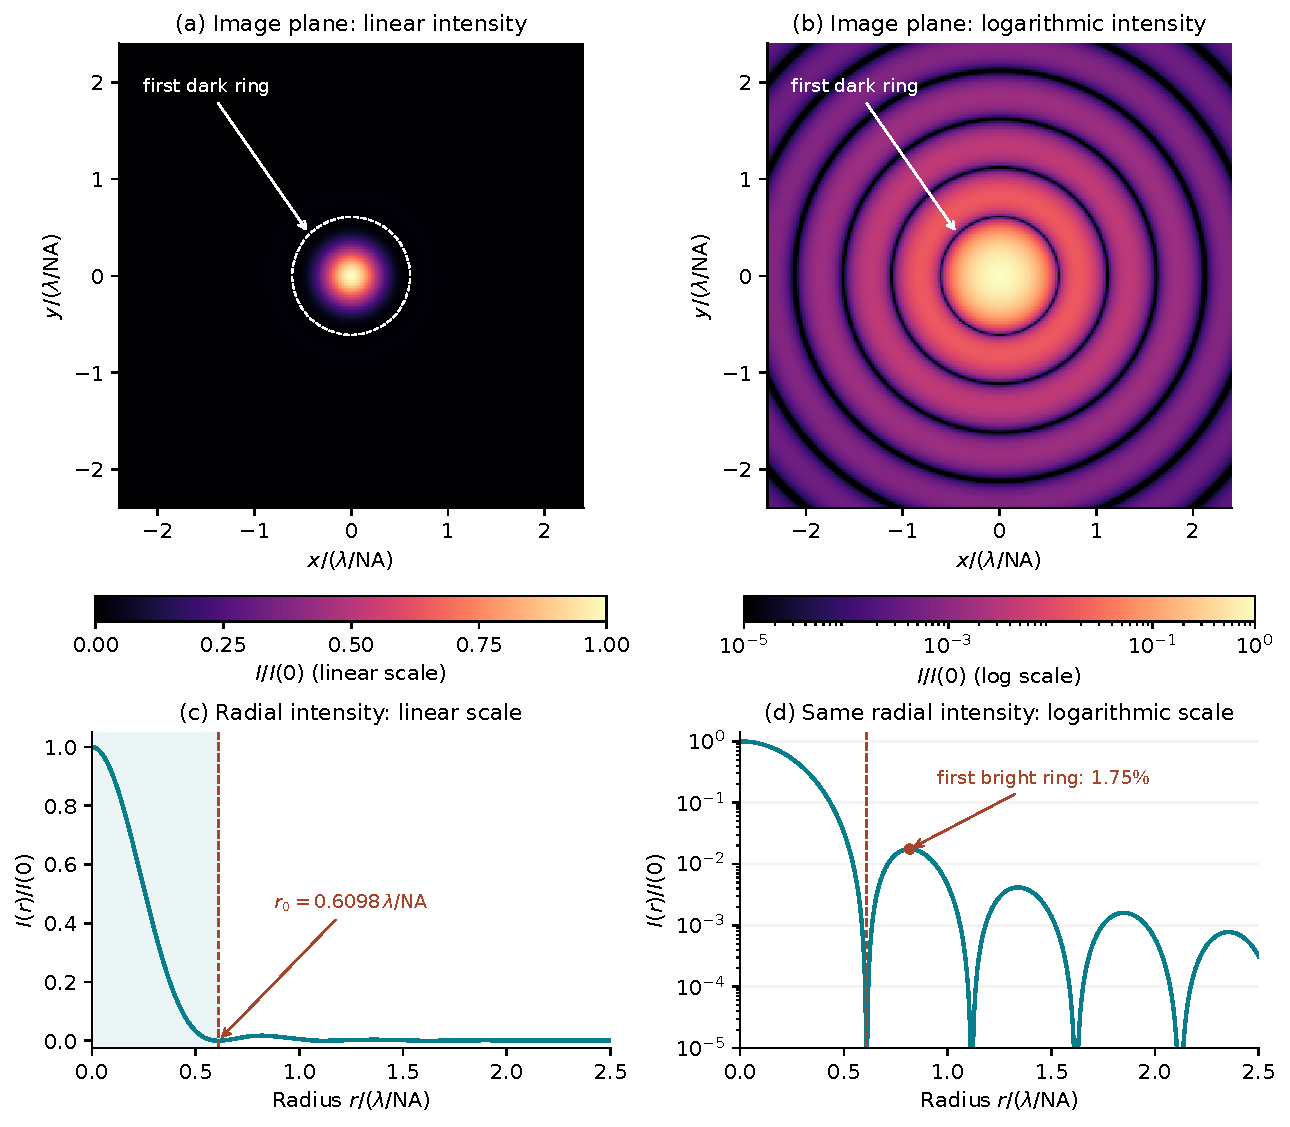
\includegraphics[width=.92\textwidth]{airy_linear_and_log.pdf}
\caption{Airy intensity for a clear circular pupil. (a,b) The same
image-plane intensity on linear and logarithmic scales; (c,d) radial
profiles. The linear panels show unlogged $I/I(0)$; absolute irradiance
requires a specified source strength. The dashed circle marks the first
dark ring. Logarithmic displays stop at $10^{-5}$; ideal minima are zero.}
\label{fig:airy}
\end{figure}

Aberration changes the phases in the pupil integral and therefore changes
the PSF, even if the pupil intensity $|P|^2$ is unchanged. A constant
phase (piston) changes no intensity; a linear pupil phase translates the
PSF; quadratic phase produces defocus. 
% For an image plane displaced
% by $\Delta z$ beyond best focus, paraxial propagation gives, after removal
% of the common phase,
% \begin{equation}
% P_{\Delta z}(\vct f)\simeq P_0(\vct f)
% \ee^{-\ii\pi\lambda\Delta z|\vct f|^2}.
% \end{equation}
% For fixed $A$, Parseval's theorem gives
% $\int|h|^2\dd^2x=\int|P|^2\dd^2f$: phase errors redistribute the
% point-image energy. They can lower the peak, distort edges, or shift
% features without changing the admitted power in this scalar model.
% The pupil and diffraction treatment follows the standard image-formation
% framework in \cite{bw,st}.
\FloatBarrier

\section{Coherence, interference averaging, and the doubled cutoff}
\subsection{Why coherent and incoherent images differ}
Take two object-point amplitudes $a_1(\tau)$ and $a_2(\tau)$ whose image
fields overlap at the \emph{same} observation point:
$U_i=a_1h_1+a_2h_2$, where $h_j=h(\vct x-M\vct x_{o,j})$.
After optical-cycle normalization, the exposure average gives
\begin{align}
I_i&=\avg{|a_1h_1+a_2h_2|^2}\notag\\
&=\avg{|a_1|^2}|h_1|^2+\avg{|a_2|^2}|h_2|^2
+2\Real\!\left[\underbrace{\avg{a_1a_2^*}}_{\Gamma_{12}}h_1h_2^*\right].
\label{eq:cross-term}
\end{align}
For fixed magnitudes, $\Gamma_{12}=A_1A_2\avg{\ee^{\ii(\phi_1-\phi_2)}}$.
A stable relative phase preserves interference. For mutually incoherent
contributions $\Gamma_{12}=0$; for example, uniformly sampled relative
phase gives $(2\pi)^{-1}\int_0^{2\pi}\ee^{\ii\phi}\dd\phi=0$.
If each contribution alone has image intensity $I_0$, their sum has
intensity $4I_0$ in phase, zero in antiphase, and $2I_0$ when mutually
incoherent. \emph{Averaging over the optical carrier alone does not remove
interference between coherent waves of the same frequency.}

For many points,
\[
I_i(\vct x)=\sum_{j,k}\avg{a_ja_k^*}h_j(\vct x)h_k^*(\vct x).
\]
Mutually incoherent object points remove all $j\ne k$ terms, leaving a
sum of intensity PSFs. Passing to a continuous object and calibrating
out the overall throughput gives
\begin{equation}
\boxed{I_{\rm incoh}=p*I_o,\qquad
p(\vct x)=\frac{|h(\vct x)|^2}{\int|h(\vct x')|^2\dd^2x'},\qquad
\int p\,\dd^2x=1.}
\label{eq:incoherent}
\end{equation}
This is linear in \emph{object intensity}; Eq.~\eqref{eq:coherent} is
linear in \emph{object field}. The same point-response shape $|h|^2$
appears in both. Coherence changes how different point responses combine.
For partial coherence the off-diagonal correlations are generally
nonzero, so neither limiting convolution alone describes the image.

\subsection{Deriving the unnormalized OTF as a pupil autocorrelation}
Define the unnormalized intensity transfer function $C$ and normalized
optical transfer function $T$ by
\begin{equation}
C(\vct q)=\FT[|h|^2](\vct q),\qquad
T(\vct q)=\frac{C(\vct q)}{C(0)}=\FT[p](\vct q).
\end{equation}
Here $\vct q$ is an \emph{intensity} spatial frequency.
Insert $h=\int P(\vct f)\ee^{\ii2\pi\vct f\cdot\vct x}\dd^2f$:
\begin{align}
C(\vct q)
&=\iint P(\vct f_1)P^*(\vct f_2)
\underbrace{\int\ee^{\ii2\pi(\vct f_1-\vct f_2-\vct q)\cdot\vct x}
\dd^2x}_{\delta^{(2)}(\vct f_1-\vct f_2-\vct q)}
\dd^2f_1\dd^2f_2\notag\\
&=\int P(\vct f)P^*(\vct f-\vct q)\dd^2f\notag\\
&=\boxed{\int P(\vct f+\vct q/2)P^*(\vct f-\vct q/2)\dd^2f.}
\label{eq:otf-autocorrelation}
\end{align}
At zero separation, Parseval's theorem yields
\begin{equation}
C(0)=\int|P(\vct f)|^2\dd^2f=\int|h(\vct x)|^2\dd^2x,
\qquad T(0)=1,\qquad
\widetilde I_i(\vct q)=T(\vct q)\widetilde I_o(\vct q).
\end{equation}
To express the autocorrelation as a convolution, define
$P^\dagger(\vct f)=P^*(-\vct f)$. Then
\begin{equation}
\boxed{C=P*P^\dagger.}
\end{equation}
It is a convolution with a \emph{conjugated and reflected} copy. For an unaberrated clear circular pupil, $P$ is real
and even, so the distinction disappears and we convolve two identical
disk indicators.

\subsection{Disk overlap explains the support and the contrast loss}
The two factors in Eq.~\eqref{eq:otf-autocorrelation} are nonzero on
disks of radius $f_c$ with centres separated by $q=|\vct q|$.
For the ideal unit-weight pupil, their product is one in the intersection
and zero elsewhere. Consequently $C(q)$ is the overlap area.
For $0\leq q\leq2f_c$, let $\theta=\cos^{-1}(q/2f_c)$.
The overlap is twice a circular sector minus its triangle:
\begin{align}
C(q)&=2\left[f_c^2\theta-
\frac q2\sqrt{f_c^2-\frac{q^2}{4}}\right],\notag\\
T(q)&=\begin{cases}
\displaystyle\frac2\pi\left[\cos^{-1}\nu-\nu\sqrt{1-\nu^2}\right],
&0\leq\nu\leq1,\\[1mm]
0,&\nu>1,
\end{cases}\qquad \nu=\frac q{2f_c}.
\label{eq:disk-otf}
\end{align}
We divided by $C(0)=\pi f_c^2$. For $q>2f_c$ there is no overlap;
at $q=2f_c$ the disks touch at one point of zero area. Thus the
incoherent intensity cutoff is $2f_c=2\NA/\lambda$.

\begin{figure}[H]
\centering
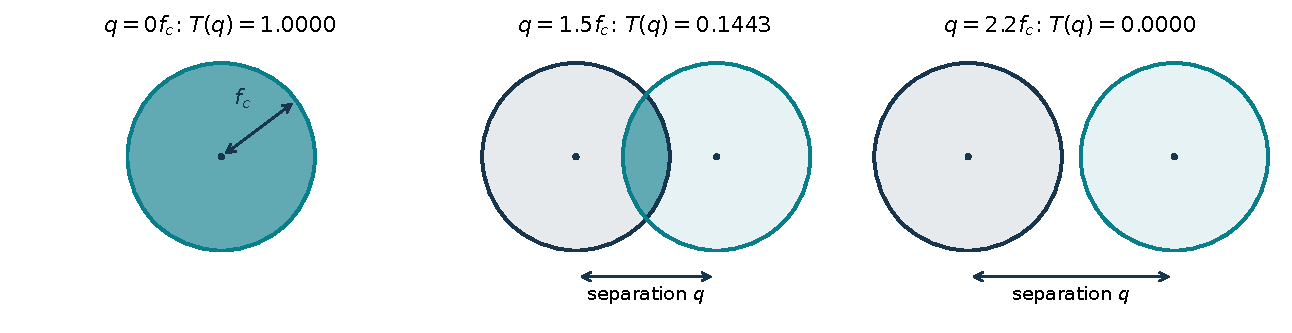
\includegraphics[width=\textwidth]{pupil_overlap.pdf}
\caption{The unnormalized OTF of a clear circular pupil is the shaded
overlap of two frequency disks, each of radius $f_c$.
Their centre separation is the intensity frequency $q$.
Dividing the overlap by $\pi f_c^2$ gives the values shown.
There is no overlap beyond $2f_c$. These disks are in spatial-frequency
space, not two physical holes in the optical system.}
\label{fig:overlap}
\end{figure}

For an aberrated pupil, overlapping points also carry the phase factor
\[
\exp\!\left\{\frac{\ii2\pi}{\lambda}
\left[W\!\left(\frac{\vct f+\vct q/2}{f_c}\right)
-W\!\left(\frac{\vct f-\vct q/2}{f_c}\right)\right]\right\}.
\]
The OTF is then a weighted complex overlap integral: phase cancellation
can reduce transfer even when the supports overlap. Its modulus
$|T|$ is the modulation transfer function (MTF); its phase describes
phase shifts of intensity modulations. A cutoff alone does not tell
us the contrast available below it.

The difference-frequency interpretation follows directly from
Eq.~\eqref{eq:otf-autocorrelation}: two admitted field components at
$\vct f_1,\vct f_2$ produce an intensity term at
$\vct q=\vct f_1-\vct f_2$. Each field frequency lies within $f_c$, but
their separation can approach $2f_c$.

% \keep{The coherent cutoff $f_c$ is the cutoff of a \emph{linear field}
% transfer function. It does not assert that a coherent intensity image
% cannot contain a $2f_c$ beat frequency. The incoherent cutoff $2f_c$
% describes \emph{linear intensity} transfer. Incoherent imaging can retain
% finer object-intensity modulation than on-axis coherent illumination in
% a specified comparison, but it is not universally better. The pupil
% has not enlarged, and neither have evanescent fields been recovered.}

\FloatBarrier
\subsection{A sinusoidal-mask example between the two cutoffs}
Use an aberration-free circular objective in air, scalar paraxial imaging
at best focus, $|M|=1$, $\lambda=500\nm$, and $\NA=0.05$. Then
$f_c=0.100\,\mu\mathrm m^{-1}$. The thin mask, uniform in $y$, has
\begin{equation}
t(x)=t_0+\epsilon\cos(2\pi qx),\qquad
t_0=0.50,\quad\epsilon=0.05,\quad q=1.5f_c,
\qquad p=1/q=6.67\um.
\label{eq:sinusoid}
\end{equation}
This is \emph{amplitude} transmission; its intensity transmission is
$|t|^2$. The mask is periodic, with no finite-edge effects.

\textbf{A: coherent, normal illumination.}
The field orders are $0,+q,-q$, with amplitudes
$t_0,\epsilon/2,\epsilon/2$. Both sidebands lie outside the pupil:
\begin{equation}
U_A=t_0P(0)+\frac\epsilon2P(q)\ee^{\ii2\pi qx}
+\frac\epsilon2P(-q)\ee^{-\ii2\pi qx}=t_0,
\qquad \boxed{I_A=0.25.}
\end{equation}

\textbf{B: an illumination giving the incoherent imaging response.}
Choose mutually incoherent plane-wave directions uniformly filling
$|\vct s|\leq3f_c$ (illumination NA $0.15$). For this three-order mask,
every source direction admitting any order lies within
$|\vct s|\leq q+f_c=2.5f_c$; the uniform source therefore covers every
relevant overlap region. After calibration, its source average gives
the full incoherent OTF for this example. This finite source need not
be spatially incoherent at every separation for every possible object.

Calibrate both cases to the response $t_0^2=0.25$ of a uniform mask
$t=t_0$. At equal incident power, B's uniform-mask throughput is $1/9$
of A's in this model, so B is divided by that factor. The comparison
concerns contrast after calibration, not photon efficiency.

Expand the object intensity and apply $T$ to its Fourier components:
\begin{align}
|t(x)|^2&=t_0^2+\frac{\epsilon^2}{2}
+2t_0\epsilon\cos(2\pi qx)
+\frac{\epsilon^2}{2}\cos(4\pi qx),\notag\\
T(q)&=\frac2\pi\left[\cos^{-1}(0.75)
-0.75\sqrt{1-0.75^2}\right]=0.144294,
\qquad T(2q)=0,\notag\\
I_B(x)&=0.25125+0.00721468\cos(2\pi qx).
\label{eq:sinusoid-result}
\end{align}
The intensity modulation at $q<2f_c$ survives; the harmonic at
$2q=3f_c$ is removed. The $\epsilon^2/2$ term explains B's slightly
higher mean. Using Michelson contrast
$\mathcal V=(I_{\max}-I_{\min})/(I_{\max}+I_{\min})$, the mask has
$19.80\%$ contrast, A has $0$, and B has $2.87\%$
(Fig.~\ref{fig:sinusoid}). This is a concrete case of higher cutoff
preserving finer periodic structure, though with strongly attenuated contrast.

\begin{figure}[H]
\centering
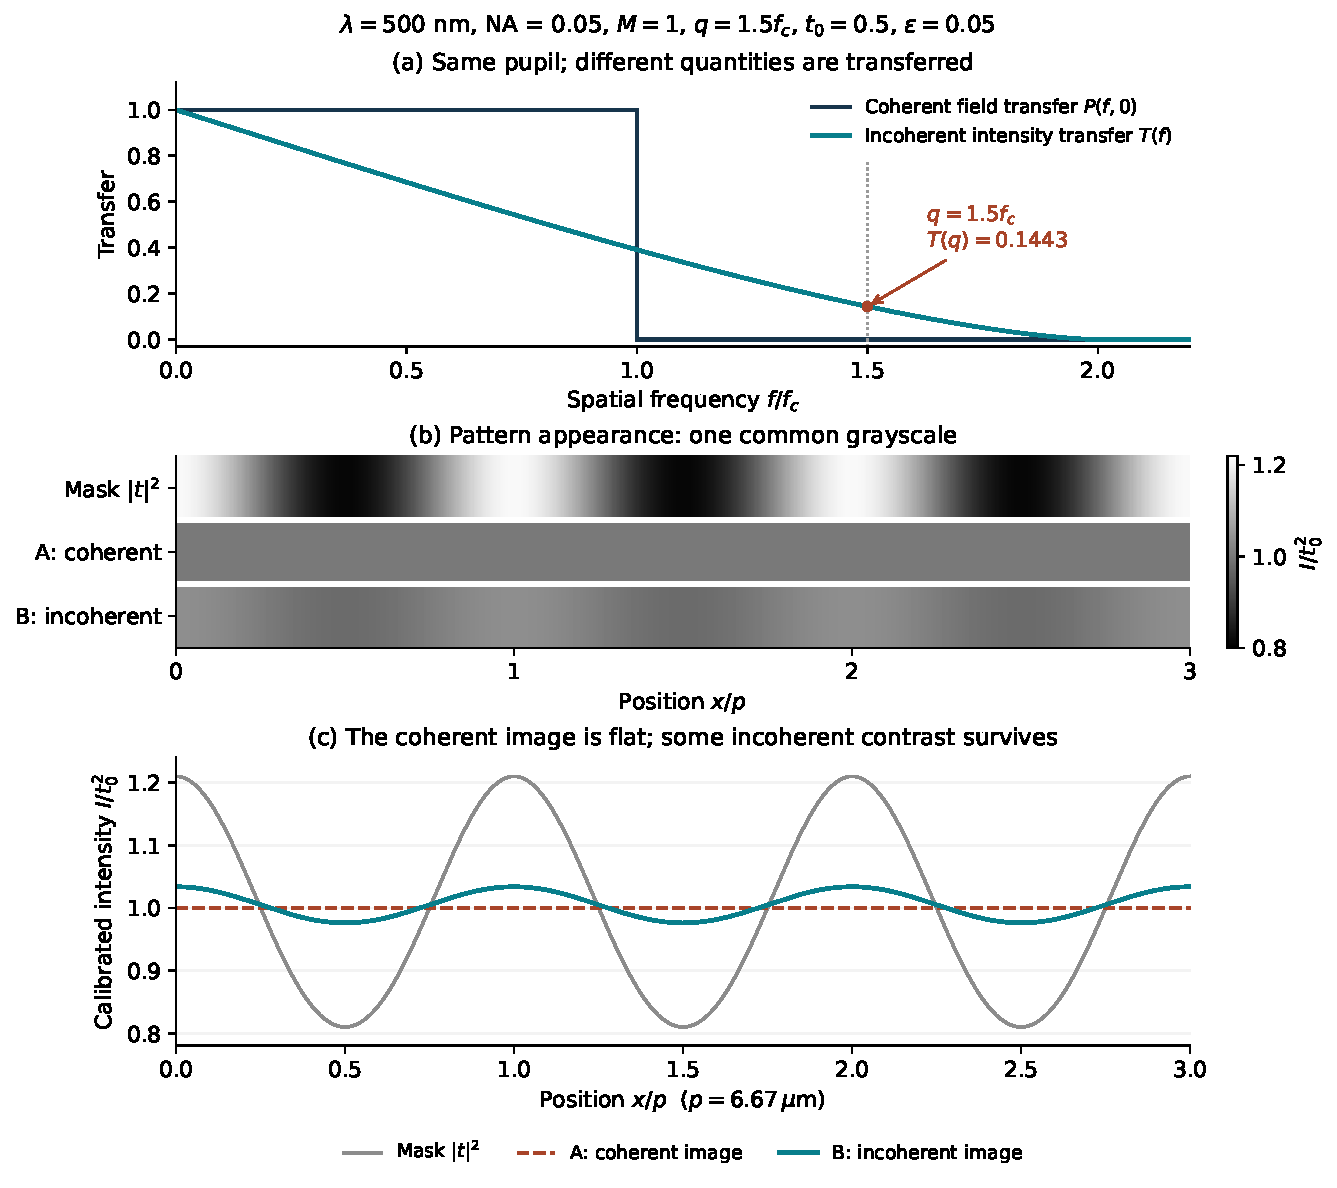
\includegraphics[width=.94\textwidth]{coherence_comparison.pdf}
\caption{Sinusoidal-mask comparison with the same objective.
(a) Coherent \emph{field} transfer and incoherent \emph{intensity} transfer.
(b) One common grayscale, without separate contrast stretching.
(c) Profiles divided by $t_0^2$ after uniform-mask calibration.
A uses normal coherent illumination; B uses mutually incoherent source
directions uniformly filling a disk of radius $3f_c$.}
\label{fig:sinusoid}
\end{figure}

To see where B's modulation comes from, a source direction
$s_x=-q/2$ places the zero and $+q$ orders at $-0.75f_c$ and $+0.75f_c$.
Both fit inside the pupil and interfere at their difference frequency
$q$. The source average retains some modulation. Appropriately oblique
\emph{coherent} illumination can also admit this pair; the result above
compares B specifically with \emph{normal} coherent illumination.


% \section{What this means for an EUV lithography optical design}
% \subsection{Sum fields within one source direction, intensities between directions}
% A useful scalar model of partial coherence assigns a nonnegative source
% weight $S(\vct s)$ to each incident plane-wave direction, normalized by
% $\int S\,\dd^2s=1$. The Fourier shift in Eq.~\eqref{eq:mask} gives
% \begin{align}
% U_{\vct s}(\vct x)
% &=\ee^{\ii2\pi\vct s\cdot\vct x}
% \int\widetilde t(\vct f)P_{\Delta z}(\vct f+\vct s)
% \ee^{\ii2\pi\vct f\cdot\vct x}\dd^2f,\notag\\
% I_i(\vct x)&=
% \int S(\vct s)
% \left|\int\widetilde t(\vct f)P_{\Delta z}(\vct f+\vct s)
% \ee^{\ii2\pi\vct f\cdot\vct x}\dd^2f\right|^2\dd^2s.
% \label{eq:source-sum}
% \end{align}
% The leading carrier has unit modulus. Equation~\eqref{eq:source-sum}
% shows the order of operations: interfere diffraction orders produced by
% \emph{one} source point, square, then add intensities from mutually
% incoherent source points. An extended angular source generally produces
% partial spatial coherence at the mask, not automatically the fully
% incoherent object model of Eq.~\eqref{eq:incoherent}.
% All frequencies here use image-equivalent coordinates.

% Changing the source moves mask orders relative to the projection pupil;
% changing NA changes its support; changing aberration changes their
% relative phases. These are separate design controls.
% The quasar illumination in Chen et al.\ is one particular angular
% distribution chosen for contact-layer imaging \cite{chen}.

% \subsection{Why the hardware is reflective, and why the mask needs Maxwell}
% At EUV wavelengths, absorption makes ordinary transmissive lens trains
% and long air paths unsuitable. A practical EUV path therefore uses
% vacuum, multilayer mirrors, and a reflective patterned mask. With the
% $\ee^{-\ii\omega t}$ convention, a passive material has
% $\widetilde n=1-\delta+\ii\beta$, $\beta>0$. A forward plane wave obeys
% \begin{equation}
% \mathcal E(z)=\mathcal E(0)
% \ee^{\ii k_0(1-\delta)z}\ee^{-k_0\beta z},\qquad
% \frac{I(z)}{I(0)}=\ee^{-4\pi\beta z/\lambda_0}.
% \end{equation}
% The intensity ratio follows from the squared amplitude decay for that
% wave in the same homogeneous material; interface fluxes still require
% the electromagnetic boundary conditions.

% A multilayer has a complex reflection coefficient
% $r=|r|\ee^{\ii\phi_r}$. Its magnitude affects throughput and its phase
% affects interference. Surface shape and alignment supply geometrical
% wavefront error, while coating thickness and incidence angle also change
% phase and amplitude. Schematically, for a pupil ray through the projector,
% \[
% P\ \propto\ \text{aperture}\times\prod_j|r_j|
% \times\exp\!\left[\ii k_0W_{\rm geom}+\ii\sum_j\phi_{r_j}\right],
% \]
% after subtracting the ideal reference phase. Thus the full pupil can
% encode the optics' imperfections, but a hardware design must calculate
% how actual mirrors and coatings generate that pupil \cite{bw,st}.

% The mask is also a three-dimensional electromagnetic scatterer. Its
% absorber height, sidewalls, multilayer, oblique incidence, and polarization
% affect the complex diffraction orders. Replacing it by one
% source-independent scalar $t(x,y)$ is then an approximation. A more
% complete source-point calculation uses Maxwell-computed order amplitudes
% $a_g(\vct s,\text{polarization})$ inside the coherent sum, then averages
% intensities as above. Evanescent near fields can affect this scattering
% even though the far-field projector does not carry them to the wafer.
% The mask chief-ray angle and the wafer-side NA cone are different angles.

% \subsection{The target is a robust printed contour}
% For the $\lambda=13.5\nm$, $\NA=0.33$ conditions used by Chen et al.,
% \begin{equation}
% f_c=0.02444\,\mathrm{nm}^{-1},\qquad
% 2f_c=0.04889\,\mathrm{nm}^{-1},\qquad
% \frac{\lambda}{\NA^2}=123.97\nm.
% \end{equation}
% The first two quantify ideal field and incoherent-intensity support.
% The third is a \emph{focus-sensitivity scale}, not a specified depth of
% focus: at the pupil edge, paraxial defocus phase is
% $|\phi_{\rm edge}|=\pi|\Delta z|\NA^2/\lambda$. Increasing NA admits
% finer detail but also increases sensitivity to focus error.

% The $24.95\nm$ Airy radius is a point-image scale, not a lower bound
% on a thresholded contact-hole width. A periodic mask, source shaping,
% and resist response determine the final contour. Hence it does not by
% itself contradict the paper's $14\nm$ target contacts \cite{chen}.

% For a simple contour model, write $D I(x_e)=\Theta$, with $I$ an aerial
% image relative to a fixed intensity reference, $D$ the corresponding
% exposure-dose scale, and $\Theta$ a threshold. Small changes give
% \begin{equation}
% \boxed{\delta x_e=-\frac{\delta I(x_e)+I(x_e)\,\delta D/D}{I'(x_e)}.}
% \label{eq:edge}
% \end{equation}
% This is an illustrative threshold model, not a complete resist model.
% It shows why intensity slope matters: the same optical or dose error
% moves a shallow edge farther. Critical dimension (CD) measures a feature
% width, pattern shift (PS) its centre displacement, and a process
% variation band (PVB) the spread of contours under prescribed focus and
% dose changes. The normalized image log slope,
% $\mathrm{NILS}=w|I'(x_e)/I(x_e)|$ for reference width $w$, measures
% relative edge steepness.

% Finally, represent an allowed pupil error as $W=\sum_jc_jZ_j$ using a
% specified Zernike basis. The physical design chain is
% \[
% \boxed{\text{hardware}\ \longrightarrow\ (A,W)
% \ \longrightarrow\ I_i\ \longrightarrow\ \text{contours}
% \ \longrightarrow\ (\mathrm{CD},\mathrm{PS},\mathrm{PVB}).}
% \]
% An aberration budget allocates tolerances so that those pattern metrics
% remain acceptable across the required operating conditions. Equal RMS
% wavefront error need not give equal imaging performance, because the
% mask and source sample different pupil regions and phase differences.
% This is the rationale for the contact-layer-specific aberration budgets
% studied by Chen et al.\ \cite{chen}. The equations above explain how
% electromagnetic fields, pupil design, and illumination enter that goal.

\newpage
\begin{thebibliography}{9}
\bibitem{bw}
M. Born and E. Wolf, \emph{Principles of Optics: Electromagnetic Theory
of Propagation, Interference and Diffraction of Light}, 4th ed.,
Pergamon Press. See \S1.3 for electromagnetic waves, \S\S1.5--1.6 for
reflection and films, \S\S8.3 and 8.5.2 for diffraction and the circular
aperture, and \S9.5 and \S10.4 for imaging and coherence.

\bibitem{st}
B. E. A. Saleh and M. C. Teich, \emph{Fundamentals of Photonics},
2nd ed., Wiley (2007). See \S\S2.1--2.2 and 2.5 for wave and paraxial
optics, \S\S4.1--4.4 for Fourier optics and image formation, and
\S6.2 for electromagnetic reflection.

\bibitem{chen}
Z. Chen, L. Dong, H. Ding, and Y. Wei,
``Aberration budget analysis of EUV lithography from the imaging
performance of a contact layer in a 5 nm technology node,''
\emph{Applied Optics} \textbf{62}(27), 7270--7279 (2023).
\href{https://doi.org/10.1364/AO.496461}{doi:10.1364/AO.496461}.
\end{thebibliography}
\end{document}
